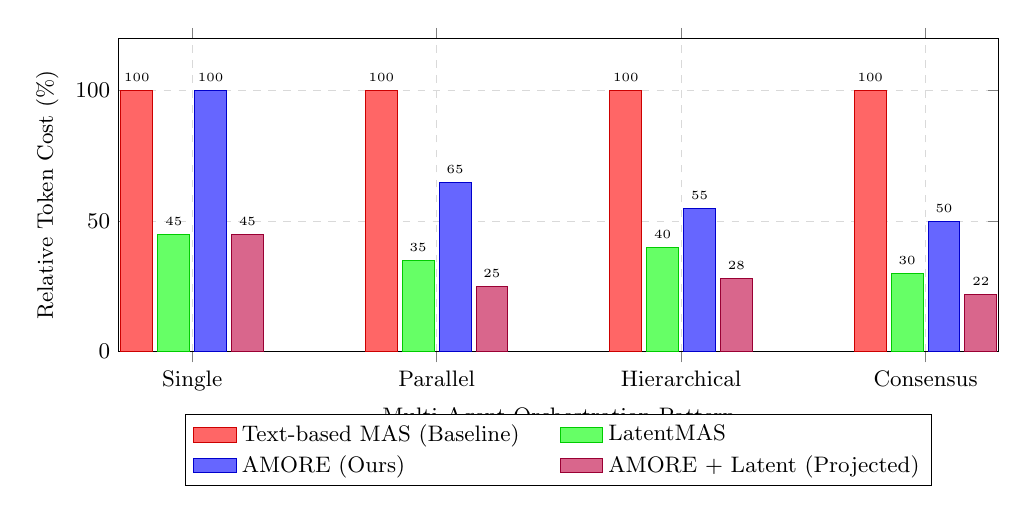
\begin{tikzpicture}[scale=0.9, transform shape]
	\begin{axis}[
		ybar,
		width=14cm,
		height=6cm,
		bar width=0.45cm,
		ylabel={Relative Token Cost (\%)},
		ylabel style={font=\small},
		xlabel={Multi-Agent Orchestration Pattern},
		xlabel style={font=\small},
		symbolic x coords={Single, Parallel, Hierarchical, Consensus},
		xtick=data,
		xticklabel style={font=\small},
		yticklabel style={font=\small},
		ymin=0,
		ymax=120,
		legend style={
			at={(0.5,-0.2)},
			anchor=north,
			legend columns=2,
			font=\small,
			/tikz/every even column/.append style={column sep=0.5cm}
		},
		legend cell align={left},
		nodes near coords,
		nodes near coords style={font=\tiny, above},
		grid=major,
		grid style={dashed, gray!30},
		area legend,
		]
		% Traditional Text-based MAS (baseline = 100%)
		\addplot[fill=red!60, draw=red!80!black] coordinates {
			(Single, 100) (Parallel, 100) (Hierarchical, 100) (Consensus, 100)
		};
		% LatentMAS (50-80% reduction)
		\addplot[fill=green!60, draw=green!80!black] coordinates {
			(Single, 45) (Parallel, 35) (Hierarchical, 40) (Consensus, 30)
		};
		% AMORE (adaptive selection)
		\addplot[fill=blue!60, draw=blue!80!black] coordinates {
			(Single, 100) (Parallel, 65) (Hierarchical, 55) (Consensus, 50)
		};
		% AMORE + Latent (projected)
		\addplot[fill=purple!60, draw=purple!80!black] coordinates {
			(Single, 45) (Parallel, 25) (Hierarchical, 28) (Consensus, 22)
		};
		\legend{Text-based MAS (Baseline), LatentMAS, AMORE (Ours), AMORE {+} Latent (Projected)}
	\end{axis}
\end{tikzpicture}